\documentclass[10pt,a4paper]{paper}
\usepackage[utf8]{inputenc}
\usepackage{graphicx}
\usepackage{subcaption}
\usepackage{enumitem}
\usepackage{tikz}
\usetikzlibrary{calc}
\usepackage{pgfgantt}
\definecolor{TableOrange}{RGB}{255,151,46}
\definecolor{TableBlue}{RGB}{38,125,184}

\newcommand{\tup}[1]{{\langle #1 \rangle}}

\pdfoptionpdfminorversion=5


\title{Artificial Intelligence for the Automated Synthesis and Validation of Programs}
\author{Sergio Jim\'enez Celorrio\\
\footnotesize Universitat Politécnica de València, Spain\\
\small Area: \underline{Ciencias de la Computación y Tecnología Informática}}

\begin{document}
\maketitle

\begin{abstract}
Programming errors, commonly known as {\em bugs}, cause undesired software behavior making a program crash or enabling malicious users to access private data. Just for 2017, the cumulative cost of software bugs is worldwide estimated in more than one trillion US dollars. 

This research project aims to investigate a novel approach for software development, that leverages Artificial Intelligence, to reduce the chances of introducing programming errors. The project proposes to address {\bf automatic program synthesis and validation starting from {\em input-output} tests cases, and using {\em AI planning} as a problem solving engine}. Our work on this particular research topic is the recipient of the {\em 2016 distinguished paper award} at {\sc IJCAI}, the main international conference on Artificial Intelligence.
\end{abstract}

\section{Historial científico-técnico del Equipo de Investigadores (Apartado 5.1,bases de la convocatoria)}

The project will be developed within the {\em Group of Reasoning on Planning and Scheduling} (GRPS){\footnote{\tt http://users.dsic.upv.es/grupos/grps/}}, that is part of the {\em Department of Computer Systems and Computation} of the UPV. In the last 10 years, the GRPS has led 3 research projects of the Spanish national research plan on {\em AI planning}. Further, the GRPS has developed its own AI planner, that is participating  at the International Planning Competition (IPC-2018).

The research group for this project comprises: 1 principal investigator, 1 senior researcher and 1 PhD student. All of them are GRPS members. 

\subsection{Principal Investigator: Sergio Jiménez Celorrio}
Sergio is a {\em Ramón y Cajal} fellow at the Universitat Politècnica de València (2017-2022). Previously, Sergio was a post-doc at the University of Melbourne and a {\em Juan de la Cierva} fellow at the Universitat Pompeu Fabra de Barcelona. From 2004 to 2013 Sergio was assistant lecturer at the Universidad Carlos III de Madrid where he obtained the {\em Distinguished Thesis Award 2011}. Sergio is co-organizer of the {\em $7^{th}$ International Planning Competition} and program committee at top international conferences on Artificial Intelligence.

His research addresses complex {\em decision-making} problems with innovative integrations of two {\em Artificial Intelligence} paradigms: {\em Machine Learning} and {\em AI Planning}. His research trajectory on this topic has produced a novel approach to the synthesis of programs, grammars and controllers for autonomous behavior and is the recipient of the {\it 2016 distinguished paper award} at the International Joint Conference on Artificial Intelligence (IJCAI)\footnote{IJCAI is ranked as {\it A+} by the CORE rank and with {\it h5-index} 43 at Google Scholar}, the main international conference on {\em Artificial intelligence}.

His top five scientific contributions are:
\begin{enumerate}
\item Inductive programming with classical planning. {\footnotesize~\cite{javi-ijcai17},~\cite{segovia2016generalized},~\cite{jimenez2015computing}}.
\item Generalization in AI planning. {\footnotesize~\cite{javi-icaps17},~\cite{damir-derived-ijcai16},~\cite{javi-fsc-ijcai16}}.
\item Learning to relieve the {\it knowledge acquisition bottleneck} in AI planning. {\footnotesize{~\cite{diego-icaps18},~\cite{jimenez2013integrating},~\cite{jimenez2008architecture},~\cite{jimenez2006planning},~\cite{lanchas2007learning}}}.
\item Machine learning for addressing the {\it curse of dimensionality} in AI planning. {\footnotesize~\cite{jimenez2012review},~\cite{de2011scaling},~\cite{de2008learning}}.  
\item Evaluation in AI planning. {\footnotesize~\cite{lopez2015deterministic},~\cite{lopez2013automating},~\cite{coles2012survey}}. 
\end{enumerate}

General quality indicators of scientific research: {\bf 373 citations} (287 since 2011) and {\bf h-index 11}. {\small\em Source google scholar}.


\subsection{Senior Researcher: Eva Onaindia} 

\subsection{Researcher in training period: Diego Aineto}


\section{Estado del arte y objetivos específicos ( Apartado 5.2.i, bases de la convocatoria)}

This research project will {\bf investigate the integration of {\em AI planning} into the {\em Test Driven Development} paradigm for the automatic synthesis and validation of programs}. Remarkably, the programs synthesized with our approach are guaranteed to be bug-free over given sets of {\em input-output} tests cases.

Here we briefly introduce the technology we will rely on along the project:
\begin{itemize}
\item {\bf AI Planning (AIP)} is the Artificial Intelligence component that studies the synthesis of sets of actions to achieve some given objectives~\cite{ghallab2004automated}. AIP arose in the late ’50s from converging studies into {\em combinatorial search}, {\em theorem proving} and {\em control theory} and now, is a well formalized paradigm for problem solving with algorithms that scale-up reasonably well. State-of-the-art planners are able to synthesize plans with hundreds of actions in seconds time~\cite{geffner2013concise}.  The mainstream approach for AIP is {\em heuristic search} with heuristics derived automatically from the problem representation~\cite{mcdermott1996heuristic,bonet2001planning}.  Current planners add other ideas to this like {\it novelty exploration}~\cite{geffner:psimulators:IJCAI17}, {\it helpful actions}~\cite{hoffmann2001ff}, {\it landmarks}~\cite{helmert2006fast}, and {\it multiqueue best-first search}~\cite{richter2010lama} for combining different heuristics.
  
\item {\bf Test driven development (TDD)}~\cite{beck:TDD:2003} is a popular paradigm for software development that is frequently used in {\it agile methodologies}~\cite{cohen2003agile}. In TDD, test cases are created before the program code is written and they are run against the code during the development, e.g. after a code change via an automated process. Tests alert programmers of bugs before handing the code off to clients (the cost of finding a bug when the code is first written is considerably lower than the cost of detecting and fixing it later). When all tests pass, the program code is considered {\em complete} while when a test fails, it pinpoints a {\em bug} that must be fixed from the program code. Tests cases are a natural form of program specification, programmers often claim {\em 'code that is difficult to test is poorly written'}. Further, writing a thorough set of tests cases forces programmers to think through inputs, outputs, and error conditions of programs. 
\end{itemize}

Now we review the two most successful approaches for program synthesis:
\begin{itemize}
\item{\bf Programming by Example (PbE)}. PbE techniques have already been deployed in the real world and are part of the {\sc Flash Fill} feature of Excel in Office 2013 that generates programs for string transformation~\cite{gulwani2011automating}. In this case the set of synthesized programs are represented succinctly in a restricted Domain-Specific Language (DSL) using a data-structure called version space algebras~\cite{mitchell1982generalization}. The programs are computed with a domain-specific search that implements a divide and conquer approach. The approach posed in this research project falls into this category.

\item In {\bf Programming by Sketching (PbS)} programmers provide a partially specified program, i.e.~a program that expresses the high-level structure of an implementation but that leaves low level details undefined to be determined by the synthesizer~\cite{solar2006combinatorial}. This form of program synthesis relies on a programming language called {\sc SKETCH}, for sketching partial programs. PbS implements a counterexample-driven iteration over a synthesize-validate loop built from two communicating SAT solvers, the inductive synthesizer and the validator, to automatically generate test inputs and ensure that the program satisfy them. Despite, in the worst case, program synthesis is harder than NP-complete, this counterexample-driven search terminates on many real problems after solving only a few SAT instances~\cite{lake2015human}.
\end{itemize}

Closely related to the aims of the project is the work on the synthesis and validation of {\it Finite State Controllers} (FSCs)~\cite{geffner:policies:IJCAI15}. The state-of-the-art algorithms for computing FSCs follow a {\it top-down} approach that interleaves {\it programming} the FSC with validating it~\cite{sergio:aprograming:ijcai16}. To keep the computation of FSCs tractable, they limit the space of possible solutions bounding the maximum size of the FSC. The computation of FSCs includes works that compile this task into another forms of problem solving so they benefit from the last advances on off-the-shelf solvers (e.g. {\em classical planning}~\cite{sergio:aprograming:icaps16}, {\em conformant planning}~\cite{Geffner:FSM:AAAI10}, {\em CSP}~\cite{Infantes:FSC:ECAI2010} or a {\em Prolog program}~\cite{Giacomo:FSM:ICAPS13}). 

Finally the generation of programs from examples is a research question also addressed in inductive Logic Programming (ILP)~\cite{muggleton1991inductive,Raedt:relationalML:book2008}. ILP arises from the intersection of {\em Machine Learning} and {\em Logic Programming} and deals with the development of inductive techniques to learn a given target concept, expressed as a  logic program,  from  examples  and  background  knowledge, that are expressed as logic facts.

(Please find the full {\em bibliography} at the end of the document)


\section{Metodología y Plan de Trabajo ( Apartado 5.2.ii, bases de la convocatoria)}
\label{subsec:metodologia}
Our current research already shows that AI planners can synthesize programs for non trivial tasks like sorting lists, traversing graphs or manipulating strings~\cite{jimenez2015computing,sergio:aprograming:icaps16,sergio:aprogramingb:ijcai16,sergio:aprograming:ijcai16}. Table~\ref{tab:programs} reports the time invested by the AI planner {\sc FD}~\cite{helmert2006fast} to solve the following programming tasks: computing the $n^{th}$ term of the {\em summatory} and  {\em Fibonacci} series, {\em reversing} a list, {\em finding} an element (and the {\em minimum} element) in a list, {\em sorting} a list or traversing a binary tree.  
 
\begin{table*}[hbt!]
  \centering
\begin{tt}  
\begin{tabular}{l@{\hspace*{30pt}}c@{\hspace*{5pt}}}
 \textbf{Programming Task} & \textbf{Time (seconds)} \\\hline
Summatory		&	1\\
Fibonacci		&	5\\
Reverse			&	22\\
Find                    &       336 \\
Minimum                 &       284 \\
Sorting			&	30\\
Tree  		&	165
\end{tabular}
\end{tt}  
\caption{\small Time to synthesize the programs with the AI planner {\sc FD}~\cite{helmert2006fast} on a processor {\em Intel Core i5 3.10GHz x 4} and with a 4GB memory bound.}
\label{tab:programs}
\end{table*}

Given a TDD programming task our approach is modeling and solving it as it were an AI planning task. Briefly, the state variables of this AIP task are {\em fluents} of the kind {\tt (var:=value)} while the initial/goal states of the AIP task encode the programming input/output tests of the TDD programming task. Finally, program instructions are encoded using two kinds of AIP actions:
\begin{enumerate}
\item {\it Programming actions}, that set an instruction on a given program line.
\item {\it Execution actions}, execute the instruction set on a given program line.
\end{enumerate}
We implement this encoding using standard planning languages, such as PDDL~\cite{fox2003pddl2}, so the AIP tasks resulting from our encoding can be solved with off-the-shelf planners, like {\sc FD}~\cite{helmert2006fast}. Interestingly, the encoding allows also program validation by (1), specifying the program to validate in the initial state of the AIP task and (2), disabling the mentioned {\it programming actions}. 

%The space of the possible programs encoded in such a way grows exponentially in the number of possible program lines. To address challenging tasks our approach must then be combined with {\em problem decomposition}. With this regard, our encoding supports callable procedures to decompose a given programming task in simpler modules and to enable recursive solutions~\cite{sergio:aprograming:icaps16,sergio:aprograming:ijcai16}. 



\subsection{Two-year workplan}
We designed a 24-month workplan plan for the {\bf development of a user-interactive program synthesizer} that (1), takes as input a set of test cases that specify the TDD programming task to solve and (2), outputs a program source code that passes these tests with a bug-free guarantee. Figure~\ref{fig:gantt} details the proposed 24-month timeline for the project.

\begin{figure}[hbt!]
\begin{ganttchart}[
  hgrid,
  group progress label node/.append style={below=3pt},
  canvas/.append style={label=below:} ]{1}{12} 
\ganttbar[bar/.append style={line width=1pt, draw=TableBlue,fill=TableBlue,fill opacity=0.6274509804}]{Design (6 months)}{1}{3} \\
\ganttbar[bar/.append style={line width=1pt, draw=TableBlue,fill=TableBlue,fill opacity=0.6274509804}]{Development (6 months)}{4}{6}\\
\ganttbar[bar/.append style={line width=1pt, draw=TableBlue,fill=TableBlue,fill opacity=0.6274509804}]{Dissemination (12 months)}{7}{12}
\end{ganttchart}
\caption{\small Workplan for the development of a user-interactive program synthesizer.}
\label{fig:gantt}
\end{figure}


\begin{enumerate}
\item {\bf T1. System design (months 1-6})
  \begin{small}
    \begin{enumerate}
    \item Design of the user-interaction for the test-case specification. Programming tasks are specified as a set of {\em input-output} tests cases plus the available instruction set. 
    \item Experimental design. Experiments will comprise taking time and memory measurements to evaluate the resources required by our approach to solve TDD programming tasks that are characterized as {\em finite state machines}.
      \item Evaluation of different AI planners available, with special attention to the planners that get the best results at the IPC-2018. 
      \end{enumerate}
  \end{small}

{\small {\bf Deliverable:} Technical report with the specifications of the system design.}
  
  \item {\bf T2. Development of the system architecture (months 7-12})
    \begin{small}
      \begin{enumerate}
      \item The programming-into-planning compiler ({\em Compiler 1}). This component parses the {\em TDD programming task} and produces an {\em AIP task} encoded in the standard planning language PDDL.
      \item The plan-into-program compiler ({\em Compiler 2}). This component extracts the program code from the solution plan produced by an off-the-shelf AI planner.
      \end{enumerate}
\end{small}      


\begin{figure}[hbt!]
\tikzstyle{block} = [draw, draw=TableBlue,fill=TableBlue,fill opacity=0.6274509804, rectangle, minimum height=3em, minimum width=6em]
\tikzstyle{input} = [coordinate]
\tikzstyle{output} = [coordinate]
\begin{center}
\begin{tikzpicture}[auto, node distance=2cm,>=latex']
    % We start by placing the blocks
    \node [input, name=input] {};
    \node [block, right of=input, node distance=4cm] (compiler1) {Compiler 1};
    \node [block, below of=compiler1, node distance=2cm] (planner) {AI Planner};    
    \node [block, below of=planner, node distance=2cm] (compiler2) {Compiler 2};
    \node [output, right of=compiler2, node distance=3cm] (output) {Program};


    % Once the nodes are placed, connecting them is easy. 
    \draw [->] (input) -- node {Programming task} (compiler1);
    \draw [->] (compiler1) -- node[] {AIP task} (planner);
    \draw [->] (planner) -- node[] {Solution plan} (compiler2);        
    \draw [->] (compiler2) -- node[] {Program}(output);
\end{tikzpicture}
\end{center}  
\caption{\small The system architecture.}
\label{fig:architecture}
\end{figure}

{\small {\bf Deliverable:} Open repository with the source code of the system architecture.}
    
\item {\bf T3. Experiments and dissemination of results (months 13-24}).
   \begin{small}
      \begin{enumerate}
      \item Reporting the experimental performance of our AIP approach for solving TDD programming tasks.
      \item Dissemination of the obtained theoretical and empirical results by submitting research papers to top international conferences and journals in AI.        
      \end{enumerate}
\end{small}        
{\small {\bf Deliverable:} Final report with the obtained conclusions and produced publications.}
\end{enumerate}


\section{Objetivos específicos del Proyecto ( Apartado 5.2.iii, bases de la convocatoria)}
\label{subsec:objectivos}

The specific objective of this project is the study of the performance of our approach for the automated synthesis and validation of programs that are characterized by these tree dimensions:
\begin{enumerate}
\item Maximum number of program lines.
\item Maximum number of program variables. 
\item Maximum size of the available instruction set.  
\end{enumerate}

In more detail, this project aims to {\bf study the performance of an Artificial Intelligence approach for the automated synthesize and validation of programs up to}: \underline{5 program lines}, \underline{50 variables with binary domain} and, an \\\underline{instruction set that comprises 10 instructions}. The performance of our approach will be evaluated with regard to the {\em computation time} and {\em memory} invested in the synthesize and validation of the programs.

Note that despite setting bounds for the programs size and kind, challenging programming tasks can be addressed using {\em problem decomposition}. With this regard, our AIP encoding already supports callable procedures to decompose a given programming task in simpler modules and to enable recursive solutions~\cite{sergio:aprograming:icaps16,sergio:aprograming:ijcai16}.

We precisely characterize the specific kind and size of the programs that we can synthesize and validate by modeling programs as {\em finite state machines}~\cite{sergio:aprograming:ijcai16}. Figure~\ref{fig:list} shows a program for traversing linked lists pictured as a {\em finite state machine}. The machine nodes mount to the different program lines while edges are tagged with a {\em condition/instruction} label, that denotes the condition under which program instructions are taken.

\begin{figure}[hbt!]
\begin{center}
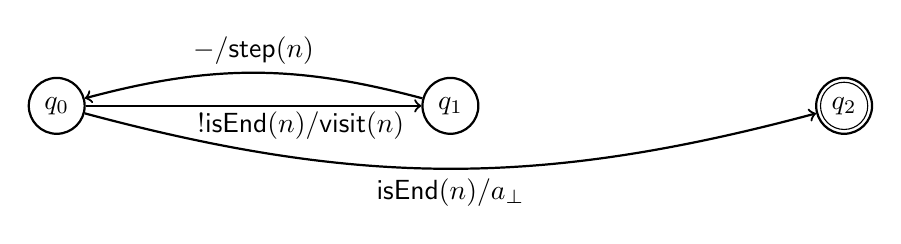
\begin{tikzpicture}
\node [thick,draw,circle] at (1,1.1) (x) {$q_0$};

\node [thick,draw,circle] at (6,1.1) (y) {$q_1$};

\node [thick,draw,circle] at (11,1.1) (z) {$q_2$};

\draw (11,1.1) circle (.3cm);

\draw [thick,->] (x) -- (y);

\draw [thick,out=345,in=195,->] (x) to (z);

\draw [thick,out=165,in=15,->] (y) to (x);

\node at (4.1,0.85) {$!\mathsf{isEnd}(n)/\mathsf{visit}(n)$};
\node at (3.5,1.8) {$-/\mathsf{step}(n)$};
\node at (6,0) {$\mathsf{isEnd}(n)/a_\bot$};
\end{tikzpicture}
\end{center}
\caption{\small {\em Finite state machine} that depicts a program to solve the programming task of traversing a linked list ($n$ is a variable that points to a node of the linked list).}
\label{fig:list}
\end{figure}

Formally, we define a program as a tuple $\tup{\mathcal{Q},q_0,Q_\bot,\mathcal{V},,\mathcal{I},\Omega,T,\Gamma}$:
\begin{itemize}
\item $\mathcal{Q}$ is a finite set of program lines where $q_0\in \mathcal{Q}$ is the {\em initial program line} and $Q_\bot\subseteq \mathcal{Q}$ is the subset of {\em terminal program lines}.
\item $\mathcal{V}$ is the finite set of program variables, where the value of each variable $v\in\mathcal{V}$ is defined in the domain $D_v$.
\item $\mathcal{I}$ is a finite instruction set where each instruction $a\in \mathcal{I}$ defines an {\em update} $\theta_a$ of a subset of the program variables.
\item $\Omega:Q\times D_{v_1}\times \ldots \times D_{v_{|\mathcal{V}|}}\mapsto\{0,1\}$ is an {\em observation function} that maps a program line and a condition over the program variables into a Boolean (1 if the condition holds 0 if  it does not). 
\item $T:Q\times\{0,1\}\rightarrow Q$ is a {\em transition function} mapping pairs of a program line and the result of a {\em condition} check into the next program line. Likewise $\Gamma:Q\times\{0,1\}\rightarrow \mathcal{I}$ is a {\em transition function} mapping pairs of a program line and the {\em condition} result into the corresponding instruction.
\end{itemize}

In the example of Figure~\ref{fig:list}, the edge $(q_0,q_2)$ with label $\mathsf{isEnd}(n)/a_\bot$ encodes that the condition is $\mathsf{isEnd}(n)?$, while $T(q_0,1)=q_2$, $\Gamma(q_0,1)=a_\bot$ encode the transition and associated instruction when $\mathsf{isEnd}(n)$ holds. The edge $(q_0,q_1)$ with label $!\mathsf{isEnd}(n)/\mathsf{visit}(n)$ encodes the transition and instruction when $\mathsf{isEnd}(n)$ does not hold, i.e.~$T(q_0,0)=q_1$ and $\Gamma(q_0,0)=\mathsf{visit}(n)$. The edge $(q_1,q_0)$ with label $-/\mathsf{step}(n)$ denotes that, when in $q_1$, the transition and instruction are always the same no matter the value of the program variables.

The {\em state of a program} is a pair $(q,s)$ that consists of the program line $q\in \mathcal{Q}$ and $s\in D_{v_1}\times \ldots \times D_{v_{|\mathcal{V}|}}$, an assignment to the variables compatible with their domains. Programs transition to a program state $(q',s')$ that is computed as follows:
\begin{enumerate}
\item First we observe whether the condition associated to the current program line holds (we denote the result of this observation as $O_q(s)\in \{0,1\}$). 
\item Then we compute the new program line $q'=T(q,O_q(s))$ and the instruction $a=\Gamma(q,O_q(s))$ to apply next. Each transition $T(q,O_q(s))$ is associated with a single observation of the variable values however, programs can represent expressive conditions including the no-op action ($a_{\bot}\in\mathcal{I}$) in the instruction set. The no-op action does not modify the program variables and affects only to the next program line which allows to concatenate conjunctions of conditions like in {\em decision trees}.
\item Finally the value of the program variables $s'=\theta_a(s)$ is updated executing the corresponding instruction $a=\Gamma(q,O(s,q))\in \mathcal{I}$.
\end{enumerate}
 



\section{Beneficios del proyecto. Difusión y Explotación en su caso de los Resultados.}
\label{subsec:beneficios}
This project will provide new insights into the current understanding of how Artificial Intelligence can assist programmers in the software development. Research in AI algorithms is too often tested with laboratory problems and AIP is not an exception. Most of the new planning algorithms are only tested within the benchmarks of the International Planing Competition~\cite{vallati:IPC:AI15}. This project will also help to meet the computational and expressiveness limits of AI planners when addressing real-world programming tasks. Promising research opportunities come from the application of AIP to {\em program synthesis} given that, {\em program synthesis} with a tests base, can also be seen as a dual to {\em program testing}. AIP has recently shown successful in {\em program testing} to generate {\em attack plans} that completed non-trivial software security tests~\cite{hoffmann2015simulated,steinmetz2016revisiting,shmaryahu2016constructing,steinmetz2016goal}.

The expected benefits of this project are:
\begin{enumerate}
\item The definition of {\bf effective metrics for assessing how well a given program covers a set of {\em input-output} test cases}.
\item An empirical {\bf study on the performance of the state-of-the-art AI planners for the {\em Synthesis and Validation of Programs}}.
\item The development, evaluation and dissemination of a finished {\bf open source software for the {\em Synthesis and Validation of Programs}}.
\end{enumerate}

Our current work on {\em program synthesis} with AIP already produced {\bf publications at top international conferences on Artificial Intelligence}~\cite{segovia2017generating,sergio:aprogramingb:ijcai16,sergio:aprograming:ijcai16,sergio:aprograming:icaps16} and is the recipient of the {\it 2016 distinguished paper award} at the International Joint Conference on Artificial Intelligence, the main international conference on {\em Artificial intelligence}. The scientific results obtained during the development of the project will be submitted to top Artificial Intelligence conferences (such as IJCAI, AAAI, ICML and ICAPS) and to the main journals in the AI field (such as AIJ, JMLR and JAIR).

\begin{tiny}
\bibliography{AI-programming}
\end{tiny}
\bibliographystyle{ieeetr}

\end{document}
